\section{Hall effect sensor (Digital and Analog)}
\begin{figure}[H]
    \centering
    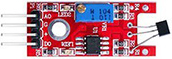
\includegraphics[angle=0, keepaspectratio=true, scale=1, width=200px, height=200px]{images/halleffect_analog_digital.jpg}
    %\caption{Caption}
\end{figure}
\subsection*{Description}
A Hall effect sensor is used to measure the magnitude of a magnetic field near the sensor module. This module has both analog and digital outputs.
\subsection*{Pin mapping}
This pin mapping corresponds to the pins from left to right with the module pins facing towards you.
\begin{table}[H]
    \centering
    \begin{tabular}{|c|c|c|c|c|}
    \hline
    Index &Label &Type &Name &Description\\ \hline
    0 &A0 &Analog output &A0 &\\ \hline
    1 &G &Ground &GND &\\ \hline
    2 &+ &Source voltage &$V+$ &Module source voltage ($5V$)\\ \hline
    3 &D0 &Digital output &D0 &\\ \hline
    \end{tabular}
    %\caption{Caption}
    %\label{tab:my_label}
\end{table}
\subsection*{Operation}
The output voltage at the analog pin (A0) is related to the magnetic field strength near the sensor. When there is no magnetic field, this output is half the supply voltage. As the ESP32 ADC can only measure voltages between 0V to 3.3V, it is recommended to supply the module with 3.3V (for larger swing). Applying a magnetic field oriented in one direction will cause the analog output voltage to be increase, the other direction will cause the voltage to decrease.

The module has a potentiometer to adjust the threshold at which the digital output pin (D0) is set to high.
\subsection*{Code}
Refer to listing \ref{python_hallsensor}.
%\lstinputlisting[caption=test]{laser.py}